\section{Results and Conclusion}

\begin{figure}[!htb]
%  \centering
%  \begin{tabular}{|c | c|}
%    \hline
%    Benchmark & P-Value
%    \\ \hline
%    asymptotics & $1.5 \times 10^{-161}$
%    \\ \hline
%    conv\_eval & $9.9 \times 10^{-261}$
%    \\ \hline
%    stlc & $8.2 \times 10^{-309}$
%    \\ \hline
%    stlc5k & $3.6 \times 10^{-305}$
%    \\ \hline
%    stlc10k & DNF
%    \\ \hline
%    stlc100k & DNF
%    \\ \hline
%    stlc\_lessimpl & $4.1 \times 10^{-311}$
%    \\ \hline
%    stlc\_lessimpl5k & $0$
%    \\ \hline
%    stlc\_lessimpl10k & DNF
%    \\ \hline
%    stlc\_small & $0$
%    \\ \hline
%    stlc\_small10k & $2.6 \times 10^{-284}$
%    \\ \hline
%    stlc\_small5k & $1.8 \times 10^{-301}$
%    \\ \hline
%  \end{tabular}
  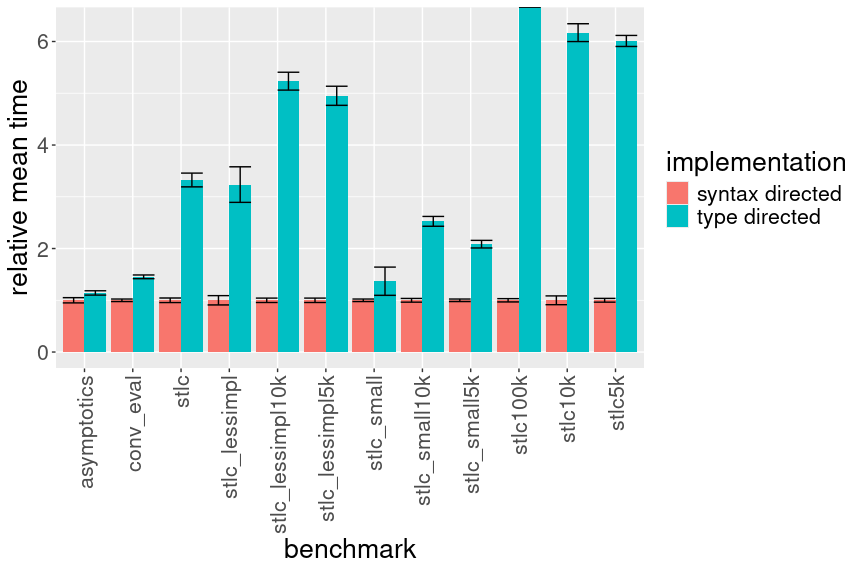
\includegraphics[totalheight=16em]{images/benchmark_graph.png}
  \caption{Benchmark Results}
  \label{fig:results}
\end{figure}

In \autoref{fig:results} we can see the results of the performance comparison between the original syntax-directed smalltt and our modified type-directed smalltt.
Each benchmark was run ten times on an AMD Ryzen 9 3900x processor with 16G of memory.
The results for each benchmark are presented so that the times for the type-directed implementation are given as a multiple of the syntax-directed times, with the syntax-directed times normalized to have a mean of 1.

Overall, the type-directed implementation performs worse, being on average 3.4 times slower than the syntax-directed implementation (excluding the benchmarks which didn't finish).
In the case of the stlc100k benchmark, the type-directed implementation failed to complete due to running out of memory.
We represent this as a column which continues off the top of the graph to infinity.
In comparison, benchmark numbers taken from equivalent benchmark suites show that Agda and Lean respectively perform 80 and 38 times slower on average than the syntax-directed smalltt implementation \citep{smalltt}.

We conjecture that the main reason for the discrepancy between the syntax and type-directed implementations, is that the syntax-directed implementation is able to take greater advantange of glued evaluation.
% Glued evaluation exploits the fact that substitution and evaluation are functions with respect to judgmental equality to speed up the judgmental equality check.
Glued evaluation exploits the fact that both substitution and evaluation respect judgmental equality to speed up the judgmental equality check.
In other words, if $\tyEqJ{\Gamma, x : A}{e}{e'}{B}$ then both $\tyEqJ{\Gamma}{\subst{e}{x}{d}}{\subst{e'}{x}{d}}{B}$ and $\tyEqJ{\Gamma}{n}{n'}{B}$ where $\steps{e}{n}$ and $\steps{e'}{n'}$.
Using these facts, we can avoid normalizing or performing a substitution on terms we are checking for equality if they are already judgmentally equal.

Glued evaluation comes to a head when comparing terms whose types contain many redexes.
Since we can only compare terms with the same type for equality, we must first compare the types of the terms, and glued evaluation lets us perform this comparison without computing many of the redexes.
In the type-directed implementation, however, we still fully normalize the type of both terms, since we need to know if it is a type at which we can apply an $\eta$ rule.

This conjecture leads us to the prediction that the performance difference between the syntax and type-directed implementations should correlate with the complexity of types used in the benchmark.
Indeed, we find that the benchmark for which the syntax and type-directed implementations are closest is the asymptotics benchmark which contains very little type-level computation, while the difference for the stlc benchmarks, which use quite complicated types to encode the syntax of the simply typed $\lambda$-calculus, is much larger.

As future work, we would like to further investigate this conjecture, and if it proves to be true, investigate if we can improve the performance of the type-directed approach.

Finally, there are other procedures for deriving a type-directed algorithm, and we'd like to integrate these into our comparison.
For example, in \citet{elabzoo}, the type of each term is calculated during normalization and then stored with the normalized term, so it can be inspected as needed during the equality check.
This approach may have different performance characteristics, but only supports the type-directed rule for Unit, using a syntax-directed method for $\Sigma$.
It's unclear whether either approach scales to other rules that require types, such as coproducts~\cite{altenkirch2001}.

% In \autoref{fig:results} we can see the results of the performance comparison between the original syntax-directed smalltt and our modified type-directed smalltt.
% The p-value is the probability that we got the observed benchmark results under the assumption that our modified version smalltt isn't slower than the original.
% Across the board this probability is very small, and so it seems likely that our modified version of smalltt is slower than the original.
% That being said, a few cases jump out in this table.
% 
% In the stlc\_lessimpl5k and stlc\_small benchmarks, the p-value is 0.
% We interpret this as a p-value so small that it can't be represented as a double-precision floating point number, since these are what we used to do the statistical test.
% 
% Our modified version of smalltt did not finish the stlc10k, stlc100k, and stlc\_lessimpl10k benchmarks due to running out of memory.
% That our implementation failed to complete some of the benchmarks isn't entirely surprising.
% smalltt includes equivalent benchmarks for some other common theorem provers such as Agda, Coq, and Idris2.
% In the performance comparison given in the README for smalltt, both Agda and Idris2 also failed to finish on the stlc100k.
% 
% This, however, doesn't detract from the fact that the original smalltt is clearly faster than our implementation.
% Therefore, we can reject our thesis statement and say that while the type-directed equality supports more rules than the syntax-directed equality, the syntax-directed equality performs better.


